\subsubsection{Backpropagation with Gradient Descent}
\label{sec:training-gradient-descent}
Due to the non-linearity in the network the minimum of the cost function cannot be computed analytically but numerically.
Hence, it is evaluated at a certain point.
Using backpropagation\cite{rumelhart1986learning}\cite{Goodfellow-et-al-2016} results in a gradient for each parameter.
Depending on these values representing the slope of the parameters, and, hence, their impact on the output, the parameters are changed to move closer to the minimum.
This optimization is done by using the gradient descent algorithm\cite{kiefer1952}\cite{robbins1951}.
\figref{fig:gradient-descent} illustrates this approach.
The gradients point into each direction of steepest ascent.
Because a minimum needs to be found, those are negated for pointing into the direction of steepest descent.
Finally, the parameters are moved along this direction.
\begin{figure}
	\centering
	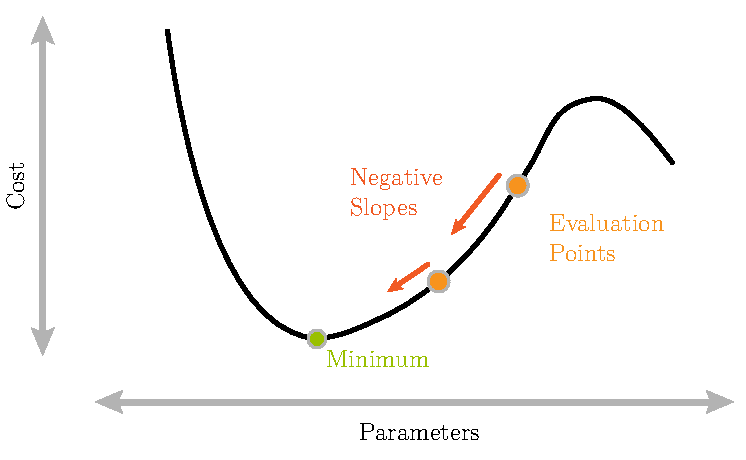
\includegraphics{images/gradient_descent.pdf}
	\caption[Schematic of Gradient Descent]{Schematic of gradient descent. Cost is evaluated, its negative gradients are computed and the parameters are moved along this direction until the minimum is reached.}
	\label{fig:gradient-descent}
\end{figure}
Following this approach means for the whole network that the cost function is backpropagated layer for layer to the beginning of the network using partial derivatives and the chain rule.
When this is completed, it is known how the parameters are influencing the output and therefore how they need to be changed depending on their slope.

Let's fill these statements with mathematical expression.
The goal of backpropagation is to compute the partial derivatives
\begin{subequations}
	\label{eq:backpropagation}
	\begin{align}
		\frac{\partial J}{\partial w^{[l]}_{jk}} &= \frac{1}{k} \sum_{i}^{k} \frac{\partial J^{(i)}}{\partial w^{[l]}_{jk}} \\
		\frac{\partial J}{\partial b^{[l]}_j} &= \frac{1}{k} \sum_{i}^{k} \frac{\partial J^{(i)}}{\partial b^{[l]}_j}
	\end{align}
\end{subequations}
of the cost function w.r.t. the parameters by averaging the partial derivatives of cost functions of $k$ samples that were passed through the network.
These $k$ samples build a batch.
\figref{fig:backpropagation-influences} recaps the data flow in a neuron in the last layer.
By checking step wise how a parameter directly influences a subsequently one, \thmref{eq:backpropagation} can be written as
\begin{subequations}
	\label{eq:backpropagation-last}
	\begin{align}
		\frac{\partial J}{\partial w^{[L]}_{jk}} &= \frac{\partial z^{[L]}_j}{\partial w^{[L]}_{jk}} \frac{\partial a^{[L]}_{j}}{\partial z^{[L]}_{j}} \frac{\partial J}{\partial a^{[L]}_{j}} \\
		\frac{\partial J}{\partial b^{[L]}_{j}} &= \frac{\partial z^{[L]}_j}{\partial w^{[L]}_{jk}} \frac{\partial a^{[L]}_{j}}{\partial z^{[L]}_{j}} \frac{\partial J}{\partial a^{[L]}_{j}}
	\end{align}
\end{subequations}
for the last layer.
How much the activations of the second to last layer influence the cost function is expressed by
\begin{equation}
	\label{eq:backpropagation-activations-last}
	\frac{\partial J}{\partial a^{[L-1]}_{k}} = \sum_{j=1}^{n_y} \frac{\partial z^{[L]}_j}{\partial a^{[L-1]}_{k}} \frac{\partial a^{[L]}_{j}}{\partial z^{[L]}_{j}} \frac{\partial J}{\partial a^{[L]}_{j}}
\end{equation}
where all weighted sums and activations of the output layer are considered.
This needs to be done because layers are fully connected and the activation of one neuron influences every neuron in the next layer.
Especially in the last layer, the activation of one neuron in the second to last layer influences directly the activations of all neurons in the last layer.
Those are directly related to the cost, which is computed by comparing them with the ground-truth values.
Hence, the influences of the activations of the neurons in the second to last layer need to be summed up.
\begin{figure}
	\centering
	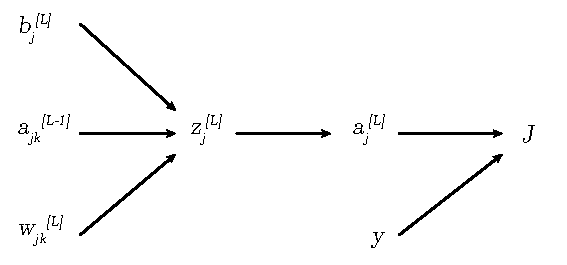
\includegraphics[]{images/backpropagation_influences.pdf}
	\caption[Data Flow in a Last-Layer Neuron for Backpropagation]{Data Flow in a Last-Layer Neuron for Backpropagation}
	\label{fig:backpropagation-influences}
\end{figure}
Once \thmref{eq:backpropagation-activations-last} is calculated for the second to last layer, this process can be repeated for all the weights and biases feeding into that layer.
This goes on layer for layer until the first one is reached.
In general,
\begin{equation}
	\label{eq:backpropagation-neuron-error}
	\delta^{[l]}_j = \frac{\partial J}{\partial a^{[l]}_j} \frac{\partial a^{[l]}_{j}}{\partial z^{[l]}_{j}}
\end{equation}
defines the error of the $j$-th neuron in the $l$-th layer.
Combining \thmref{eq:backpropagation-last} and \thmref{eq:backpropagation-neuron-error} yields
\begin{subequations}
	\label{eq:backpropagation-general}
	\begin{align}
		\frac{\partial J}{\partial w^{[l]}_{jk}} &= \frac{\partial z^{[l]}_j}{\partial w^{[l]}_{jk}} \frac{\partial a^{[l]}_{j}} {\partial z^{[l]}_{j}} \frac{\partial J}{\partial a^{[l]}_j} = \frac{\partial z^{[l]}_j}{\partial w^{[l]}_{jk}} \delta^{[l]}_j \\
		\frac{\partial J}{\partial b^{[l]}_{j}} &= \frac{\partial z^{[l]}_j}{\partial b^{[l]}_{j}} \frac{\partial a^{[l]}_{j}} {\partial z^{[l]}_{j}} \frac{\partial J}{\partial a^{[l]}_j} = \frac{\partial z^{[l]}_j}{\partial b^{[l]}_{j}} \delta^{[l]}_j
	\end{align}
\end{subequations}
as the general expressions for backpropagation where
\begin{subequations}
	\begin{align}
		\frac{\partial z^{[l]}_j}{\partial w^{[l]}_{jk}} &= a^{[l-1]}_j \\
		\frac{\partial z^{[l]}_j}{\partial b^{[l]}_j} &= 1 \\
		\frac{\partial a^{[l]}_{j}}{\partial z^{[l]}_{j}} &= \phi'(z^{[l]}_j)
	\end{align}
\end{subequations}
are the derivatives.
Summarizing the gradients of the cost function yields the compact representation
\begin{equation}
	\label{eq:cost-gradient}
	\nabla \vec{J} =
	\begin{pmatrix}
		\frac{\partial J}{\vec{W^{[1]}}} &
		\frac{\partial J}{\vec{b^{[1]}}} &
		\frac{\partial J}{\vec{W^{[2]}}} &
		\frac{\partial J}{\vec{b^{[2]}}} &
		\cdots &
		\frac{\partial J}{\vec{W^{[L]}}} &
		\frac{\partial J}{\vec{b^{[L]}}}
	\end{pmatrix}^T
\end{equation}
containing the influences of all parameters.
Each element points into its direction of steepest ascent with a magnitude.
Hence, each gradient is inverted for pointing into its direction of steepest descent for finding a minimum.
Along each direction depending on its magnitude each parameter is changed.
This can be expressed by
\begin{subequations}
	\label{eq:learning-rate}
	\begin{align}
		w^{[l]}_{jk}(\tau + 1) &= w^{[l]}_{jk}(\tau) - \gamma \nabla \vec{J}(w^{[l]}_{jk}(\tau)) \\
		b^{[l]}_j(\tau + 1) &= b^{[l]}_j(\tau) - \gamma \nabla \vec{J}(b^{[l]}_j(\tau))
	\end{align}
\end{subequations}
where the hyperparameter $\gamma$ is the learning rate and $\tau$ the iteration step.
This update procedure is done for every batch that is passed through the network.
The updates resulting from a batch are called an iteration.
This is repeated for the whole training set, which is called an epoch.
The objective of the learning rate is to control how much the parameters are adjusted.
The smaller it is, the slower the parameters are moving along the graph to the minimum.
On its way, the slope steadily gets smaller which intensifies this effect.
A similar effect arises by moving over plateaus.
Surely, the minimum will be found more exactly than with a large learning rate, but it would make learning really slow.
However, a large learning rate can steadily overshoot the minimum leading to no convergence.
These effects are illustrated in \figref{fig:learning-rate}.
Thus, a trade-off must be found or an adaption of the learning rate to certain circumstances like the magnitude of the slope is necessary.
\begin{figure}
	\centering
	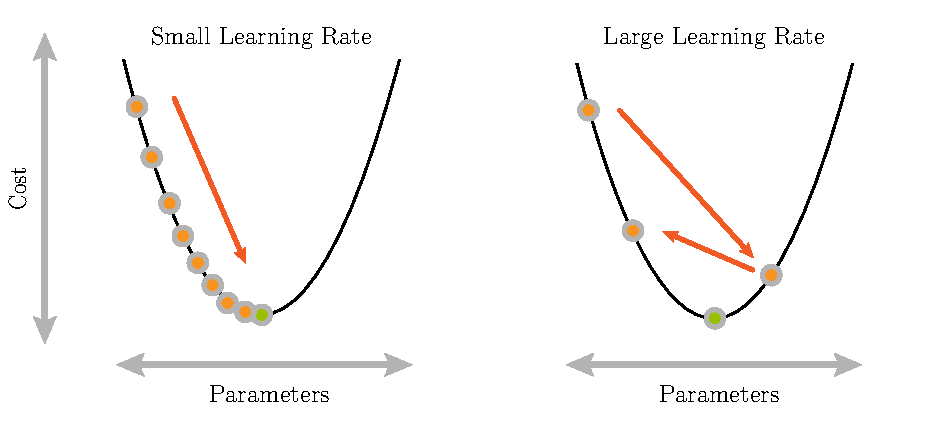
\includegraphics[]{images/gradient_descent_learning_rate.pdf}
	\caption[Comparison of Learning Rates]{Comparison of Learning Rates. A small learning rate finds the minimum slowly but more exactly than a high learning rate. However, the latter tends to overshoot the minimum.}
	\label{fig:learning-rate}
\end{figure}
According to \textit{Bengio} \cite{DBLP:journals/corr/abs-1206-5533} a traditional default value for the learning rate is $\gamma_0 = 0.1$ or $\gamma_0 = 0.01$ for standard multilayer neural networks.
However, "it would be foolish to rely exclusively on this default value".
The learning rate should be greater than $10^{-6}$ and less than $1.0$.
\textit{Goodfellow et al.} \cite{Goodfellow-et-al-2016} state, "in practice, it is common to decay the learning rate linearly until iteration $\tau$. After iteration $\tau$ it is common to leave [the learning rate] constant."
The underlying idea is to move quickly to close proximity to the minimum and then carefully to it.
Another common approach is an exponential decay like
\begin{equation}
	\gamma(\tau) = \gamma_0 \exp(-k\tau)
\end{equation}
where $\gamma_0$ is the initial learning rate, $k$ a factor and $\tau$ the time step.
The concept of changing the learning rate over time is called learning rate schedule. Its values are arbitrary and do not inevitably need to be results of a decay but can be fixed values that are active depending on the time step $\tau$, for example.

Due to the number of parameters and the use of hidden layers, cost functions are highly dimensional and neither convex nor concave.
An explanation for the latter is, that several combinations of parameters can result in the same loss value.
Hence, there are several local minima in the cost function.
According to \textit{Choromanska et al.}\cite{DBLP:journals/corr/ChoromanskaHMAL14} almost all local minima have very similar function values to the global minimum.
Hence, finding a local one is sufficient.
Having neither a convex nor concave cost function, the function probably has saddle points.
These points are no optimum, but have a gradient of $\nabla \vec{J} = \vec{0}$.
The types of critical points are shown in \figref{fig:critical-points}.
\begin{figure}
	\centering
	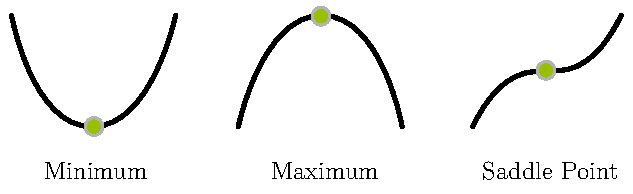
\includegraphics[]{images/gradient_descent_types.pdf}
	\caption{Types of Critical Points}
	\label{fig:critical-points}
\end{figure}
With this gradient the algorithm would get stuck.
Hence, adding some noise to \thmref{eq:learning-rate} yields
\begin{subequations}
	\begin{align}
		w^{[l]}_{jk} &:= w^{[l]}_{jk} - \gamma \nabla \vec{J}(w^{[l]}_{jk}) + \vec{\epsilon}(w^{[l]}_{jk}) \\
		b^{[l]}_j &:= b^{[l]}_j - \gamma \nabla \vec{J}(b^{[l]}_j) + \vec{\epsilon}(b^{[l]}_j)
	\end{align}
\end{subequations}
where $\vec{\epsilon}$ is a noise vector with mean 0.
Because saddle points are very unstable, adding some noise helps to overcome them.